\documentclass[12pt]{article}
\usepackage[english]{babel}
\usepackage[utf8x]{inputenc}
\usepackage{amsmath}
\usepackage{tikz}
\usetikzlibrary{arrows,automata}
\begin{document}

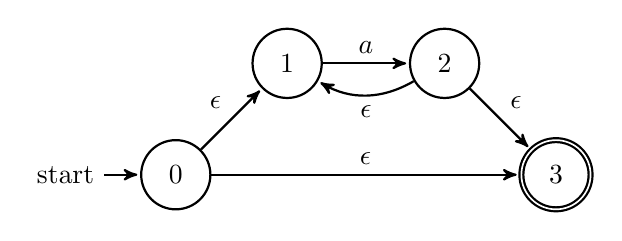
\begin{tikzpicture}[->,>=stealth',shorten >=1pt,auto,node distance=2cm,
    thick,base node/.style={circle,draw,minimum size=8pt}, real node/.style={double,circle,draw,minimum size=17pt}]

  \node[state]          (a){$1$};
  \node[state,initial]  (start) [below left of=a]{$0$};
  \node[state]          (b) [right of=a] {$2$};
  \node[state,accepting]  (c)  [below right of=b] {$3$};
  \path (start) edge node {$\epsilon$} (a)
        (a) edge    node {$a$} (b)
        (start) edge node {$\epsilon$} (c)
        (b) edge [bend left] node {$\epsilon$} (a)
        (b) edge      node {$\epsilon$} (c)
         ;
\end{tikzpicture}
\end{document}